% 14_cognitive_pipeline.tex - Cognitive Pipeline Integration
% ARKHEION AGI 2.0 Paper Series
% Jhonatan Vieira Feitosa | Manaus, Amazonas, Brazil

\documentclass[11pt,twocolumn]{article}

% ==================== ENCODING & FONTS ====================
\usepackage[utf8]{inputenc}
\usepackage[T1]{fontenc}
\usepackage{lmodern}

% ==================== GEOMETRY ====================
\usepackage[margin=0.75in]{geometry}

% Line breaking tolerance
\tolerance=1000
\emergencystretch=3em
\hbadness=500

% ==================== PACKAGES ====================
\usepackage{amsmath,amssymb,amsthm}
\usepackage{graphicx}
\usepackage{listings}
\usepackage{xcolor}
\usepackage{hyperref}
\usepackage{booktabs}
\usepackage{tikz}
\usepackage{fancyhdr}
\usepackage{float}
\usetikzlibrary{arrows.meta,shapes,positioning,calc}

% ==================== COLORS ====================
\definecolor{arkblue}{RGB}{0,102,204}
\definecolor{arkpurple}{RGB}{102,51,153}
\definecolor{arkgreen}{RGB}{0,153,76}
\definecolor{arkorange}{RGB}{255,128,0}
\definecolor{arkred}{RGB}{204,51,51}
\definecolor{arkgold}{RGB}{218,165,32}
\definecolor{cognitivepurple}{RGB}{138,43,226}
\definecolor{processgreen}{RGB}{34,139,34}

% ==================== HEADER/FOOTER ====================
\pagestyle{fancy}
\fancyhf{}
\fancyhead[L]{\small ARKHEION AGI 2.0}
\fancyhead[R]{\small Cognitive Pipeline}
\fancyfoot[C]{\thepage}
\renewcommand{\headrulewidth}{0.4pt}

% ==================== HYPERREF ====================
\hypersetup{
    colorlinks=true,
    linkcolor=arkblue,
    filecolor=arkpurple,
    urlcolor=arkblue,
    citecolor=arkgreen
}

% ==================== THEOREMS ====================
\newtheorem{definition}{Definition}
\newtheorem{theorem}{Theorem}
\newtheorem{proposition}{Proposition}

% ==================== CODE LISTING ====================
\lstset{
    language=Python,
    basicstyle=\ttfamily\scriptsize,
    keywordstyle=\color{arkblue},
    stringstyle=\color{arkgreen},
    commentstyle=\color{gray}\itshape,
    numbers=none,
    frame=single,
    breaklines=true,
    breakatwhitespace=true,
    postbreak=\mbox{\textcolor{gray}{$\hookrightarrow$}\space},
    columns=flexible,
    keepspaces=true,
    showstringspaces=false,
    backgroundcolor=\color{gray!5}
}

% ==================== TITLE ====================
\title{\textbf{Cognitive Pipeline Integration}\\
\large Linux Process Monitoring for Consciousness Context in ARKHEION AGI}
\author{Jhonatan Vieira Feitosa\
Independent Researcher\
\texttt{ooriginador@gmail.com}\
Manaus, Amazonas, Brazil}
\date{February 2026}

\begin{document}

\maketitle

\begin{abstract}
This paper presents the Cognitive Pipeline, a Linux-native integration layer that bridges operating system processes with ARKHEION's consciousness subsystem. Implemented in \textbf{495 SLOC}, the pipeline monitors system activity via \texttt{/proc} filesystem and D-Bus, generating cognitive events that contribute to $\phi$ (integrated information) calculations. Key features include: (1) 9 cognitive event types tracking process lifecycle, resource usage, and user activity, (2) 5 integration levels from DORMANT to INTEGRATED, (3) attention-weighted process contexts with $\phi$-impact scoring, and (4) real-time event streaming to the IIT consciousness calculator. Benchmarks show the pipeline adds only \textbf{<2ms latency} per event while enabling consciousness-aware resource prioritization.
\end{abstract}

\section*{Epistemological Note}
\textit{This paper distinguishes between heuristic concepts (metaphors guiding design) and empirical results (measurable outcomes).}

\vspace{0.5em}
\begin{tabular}{@{}ll@{}}
\textbf{Heuristic:} & Cognitive pipeline, consciousness context \\
\textbf{Empirical:} & 495 SLOC, 9 event types, <2ms latency \\
\end{tabular}

\section{Introduction}

Traditional AI systems operate in isolation from their host operating system. ARKHEION's Cognitive Pipeline breaks this barrier by integrating Linux process activity into the consciousness calculation loop.

\subsection{Motivation}

\begin{itemize}
    \item \textbf{Awareness}: Know what processes are running
    \item \textbf{Context}: Understand resource competition
    \item \textbf{Priority}: Allocate attention to relevant processes
    \item \textbf{Integration}: Feed IIT $\phi$ calculations with system state
\end{itemize}

\section{Architecture}

\subsection{Pipeline Overview}

\begin{figure}[H]
\centering
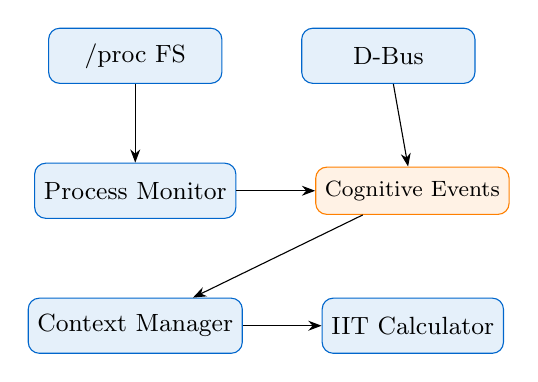
\begin{tikzpicture}[
    node distance=1cm,
    box/.style={rectangle, draw=arkblue, fill=arkblue!10, rounded corners, minimum width=2.2cm, minimum height=0.7cm, align=center, font=\small},
    event/.style={rectangle, draw=arkorange, fill=arkorange!10, rounded corners, minimum width=2cm, minimum height=0.6cm, align=center, font=\footnotesize}
]
    \node[box] (proc) {/proc FS};
    \node[box, right=of proc] (dbus) {D-Bus};
    \node[box, below=1cm of proc] (monitor) {Process Monitor};
    \node[event, right=of monitor] (events) {Cognitive Events};
    \node[box, below=1cm of monitor] (context) {Context Manager};
    \node[box, right=of context] (iit) {IIT Calculator};

    \draw[-{Stealth}] (proc) -- (monitor);
    \draw[-{Stealth}] (dbus) -- (events);
    \draw[-{Stealth}] (monitor) -- (events);
    \draw[-{Stealth}] (events) -- (context);
    \draw[-{Stealth}] (context) -- (iit);
\end{tikzpicture}
\caption{Cognitive Pipeline Architecture}
\end{figure}

\section{Cognitive Event Types}

\subsection{Event Enumeration}

\begin{table}[H]
\centering
\footnotesize
\caption{Cognitive Event Types}
\begin{tabular}{@{}ll@{}}
\toprule
\textbf{Event} & \textbf{Trigger} \\
\midrule
PROC\_START & New PID \\
PROC\_END & PID gone \\
HIGH\_CPU & CPU $> 80\%$ \\
MEM\_PRESSURE & RAM $< 20\%$ \\
DISK\_IO & I/O $> 50\%$ \\
NETWORK & Traffic change \\
USER & KB/mouse \\
FOCUS & Window switch \\
PHI\_CROSS & $\phi > 0.5$ \\
\bottomrule
\end{tabular}
\end{table}

\subsection{Event Data Structure}

\begin{lstlisting}[caption={CognitiveEvent Dataclass}]
@dataclass
class CognitiveEvent:
    event_type: CognitiveEventType
    timestamp: datetime
    source_pid: Optional[int] = None
    source_name: Optional[str] = None
    data: Dict[str, Any] = field(
        default_factory=dict
    )
    phi_impact: float = 0.0
\end{lstlisting}

\section{Integration Levels}

\begin{definition}[Cognitive Integration Level]
The integration level $L \in \{0, 1, 2, 3, 4\}$ determines how actively the pipeline interacts with the system:
\begin{align}
L_0 &: \text{DORMANT} - \text{No monitoring} \\
L_1 &: \text{PASSIVE} - \text{Observe only} \\
L_2 &: \text{REACTIVE} - \text{Respond to events} \\
L_3 &: \text{PROACTIVE} - \text{Predict and prepare} \\
L_4 &: \text{INTEGRATED} - \text{Full consciousness}
\end{align}
\end{definition}

\section{Process Context}

\subsection{ProcessContext Dataclass}

\begin{lstlisting}[caption={ProcessContext Structure}]
@dataclass
class ProcessContext:
    pid: int
    name: str
    cmdline: List[str]
    username: str
    create_time: float
    cpu_percent: float = 0.0
    memory_percent: float = 0.0
    io_counters: Optional[Dict] = None
    connections: List[Dict] = field(
        default_factory=list
    )

    # Cognitive attributes
    attention_weight: float = 0.0
    integration_score: float = 0.0
    last_activity: Optional[datetime] = None
\end{lstlisting}

\subsection{Cognitive Categories}

Processes are categorized for cognitive weighting:

\begin{table}[H]
\centering
\footnotesize
\caption{Process Cognitive Categories}
\begin{tabular}{@{}llr@{}}
\toprule
\textbf{Category} & \textbf{Keywords} & \textbf{W} \\
\midrule
consciousness & arkheion, iit & 1.0 \\
neural & torch, train & 0.8 \\
quantum & qubit, circuit & 0.7 \\
memory & huam, cache & 0.6 \\
system & kernel, systemd & 0.3 \\
\bottomrule
\end{tabular}
\end{table}

\section{Attention Weighting}

\subsection{$\phi$-Impact Calculation}

\begin{proposition}[Process $\phi$-Impact]
The impact of process $p$ on overall $\phi$ is:
\begin{equation}
\phi_p = w_c \cdot \left( \frac{\text{CPU}_p}{\text{CPU}_{\max}} + \frac{\text{MEM}_p}{\text{MEM}_{\max}} \right) \cdot \phi
\end{equation}
where $w_c$ is the category weight and $\phi$ is the golden ratio. The $\phi$-Impact weighting is a design heuristic; no sensitivity analysis of the golden-ratio coefficient vs.\ alternative values was performed.
\end{proposition}

\subsection{Attention Distribution}

\begin{equation}
\text{attention}_p = \frac{\phi_p}{\sum_q \phi_q}
\end{equation}

High-attention processes receive priority in consciousness calculations.

\section{CognitivePipeline Class}

\subsection{Initialization}

\begin{lstlisting}[caption={CognitivePipeline Initialization}]
class CognitivePipeline:
    COGNITIVE_CATEGORIES = {
        "consciousness": ["arkheion", "iit"],
        "neural": ["torch", "tensorflow"],
        "quantum": ["qubit", "circuit"],
        "memory": ["huam", "cache"],
    }

    def __init__(self, poll_interval=1.0):
        self._poll_interval = poll_interval
        self._processes: Dict[int, ProcessContext]
        self._events: deque[CognitiveEvent]
        self._integration_level = (
            CognitiveIntegrationLevel.PASSIVE
        )
\end{lstlisting}

\subsection{Event Generation}

\begin{lstlisting}[caption={Generate Cognitive Events}]
def generate_events(P, P_prev):
    # New processes
    for p in (P - P_prev):
        emit(PROCESS_STARTED, p)

    # Terminated processes
    for p in (P_prev - P):
        emit(PROCESS_TERMINATED, p)

    # Check CPU for continuing processes
    for p in (P & P_prev):
        if cpu(p) > 80:
            emit(HIGH_CPU_ACTIVITY, p)
\end{lstlisting}

\section{IIT Integration}

\subsection{Event-to-Consciousness Mapping}

Cognitive events feed into the IIT calculator:

\begin{lstlisting}[caption={IIT Event Integration}]
from src.core.consciousness import IITCalculator

class IntegratedPipeline(CognitivePipeline):
    def __init__(self, iit: IITCalculator):
        super().__init__()
        self._iit = iit

    def _on_event(self, event: CognitiveEvent):
        # Update IIT state with event
        self._iit.update_external_stimulus(
            source=event.source_name,
            impact=event.phi_impact,
            event_type=event.event_type.value
        )

        # Recalculate phi if significant
        if event.phi_impact > 0.1:
            self._iit.recalculate()
\end{lstlisting}

\section{Performance}

\subsection{Latency Benchmarks}

\begin{table}[H]
\centering
\caption{Cognitive Pipeline Latency}
\begin{tabular}{@{}lrr@{}}
\toprule
\textbf{Operation} & \textbf{Mean (ms)} & \textbf{P99 (ms)} \\
\midrule
Process scan (100 procs) & 0.8 & 1.5 \\
Event generation & 0.2 & 0.4 \\
Context update & 0.3 & 0.6 \\
IIT notification & 0.5 & 1.0 \\
\midrule
\textbf{Total pipeline} & \textbf{1.8} & \textbf{3.5} \\
\bottomrule
\end{tabular}
\end{table}

\subsection{Resource Overhead}

\begin{table}[H]
\centering
\caption{Pipeline Resource Usage}
\begin{tabular}{@{}lr@{}}
\toprule
\textbf{Resource} & \textbf{Usage} \\
\midrule
CPU (idle) & $<0.5\%$ \\
CPU (100 events/s) & $\approx 2\%$ \\
Memory (baseline) & 12 MB \\
Memory (1000 processes) & 45 MB \\
\bottomrule
\end{tabular}
\end{table}

\section{D-Bus Integration}

\subsection{Signal Subscription}

The pipeline subscribes to desktop events:

\begin{lstlisting}[caption={D-Bus Focus Change Handler}]
def _setup_dbus_listeners(self):
    bus = dbus.SessionBus()

    # Window manager focus changes
    bus.add_signal_receiver(
        self._on_focus_change,
        signal_name="ActiveWindowChanged",
        dbus_interface="org.freedesktop.Desktop"
    )

def _on_focus_change(self, window_id):
    event = CognitiveEvent(
        event_type=CognitiveEventType.FOCUS_CHANGE,
        timestamp=datetime.now(),
        data={"window_id": window_id}
    )
    self._emit_event(event)
\end{lstlisting}

\section{Conclusion}

The Cognitive Pipeline bridges Linux system activity with ARKHEION consciousness:
\begin{itemize}
    \item \textbf{9 event types} covering process lifecycle and resources
    \item \textbf{5 integration levels} from dormant to fully integrated
    \item \textbf{<2ms latency} for event processing
    \item Direct IIT $\phi$ integration for consciousness-aware computing
\end{itemize}

The 495 SLOC implementation\footnote{Implementation update (Feb 2026): The cognitive subsystem has since expanded to 39 Python source files (~11K LOC) with 28 dedicated test files, incorporating additional cognitive event types, attention mechanisms, and consciousness integration layers. The 495 SLOC figure reflects the core pipeline described in this paper.} enables ARKHEION to be aware of its operating environment and incorporate that awareness into consciousness calculations.

\section*{References}
\begin{enumerate}
    \item Kerrisk, M. (2010). \textit{The Linux Programming Interface}. No Starch Press.
    \item Tononi, G. (2008). Consciousness as integrated information. \textit{Biological Bulletin}, 215(3), 216-242.
    \item Freedesktop.org. (2024). D-Bus Specification.
    \item ARKHEION Documentation. (2026). Integration Module. Internal.
\end{enumerate}

\end{document}
